% Reuse the opening report cutout, with a skimmable safety scope above it.
\begin{tikzpicture}[remember picture,overlay,
  every node/.style={anchor=west,inner sep=0pt,font=\normalsize,text=Ink}]
\begin{scope}[shift={(current page.south west)}]
  \node at (.65,7.0) {\textbf{About 40 pages} on safety training and evaluations};
  % One table with aligned columns, soft row fills, and shared padding.
  \path[fill=Pale!70] (.65,6.15) rectangle (15.35,3.35);
  \path[fill=Pale!35] (.65,5.22) rectangle (15.35,4.28);
  \draw[Ink!12,line width=.45pt] (.65,5.22) -- (15.35,5.22);
  \draw[Ink!12,line width=.45pt] (.65,4.28) -- (15.35,4.28);
  \node at (.9,5.685) {\textbf{Systemic risks}};
  \node at (3.85,5.685) {\color{Muted}Biological and chemical weapons, loss of control, cyber offense};
  \node at (.9,4.75) {\textbf{Model behavior}};
  \node at (3.85,4.75) {\color{Muted}Conversations, agents, over-refusal, prompt injection, and child safety};
  \node at (.9,3.815) {\textbf{Evaluations}};
  \node at (3.85,3.815) {\color{Muted}Independent evaluations and human and automated red-teaming};
  \node[anchor=south west] at (.65,.15)
    {\begin{minipage}{14.7cm}% Shared cutout used both to introduce Beam and to close the Beam section.
\begin{center}
\begin{tikzpicture}
  \path[use as bounding box] (0,0) rectangle (14.7,2.4);
  \clip (0,0) rectangle (14.7,2.4);
  \fill[black!10] (2.55,-.1) rectangle (12.35,2.28);
  \node[anchor=north,inner sep=0pt] at (7.4,2.35)
    {\href{https://reflection.ai/documents/beam-model-tech-report}{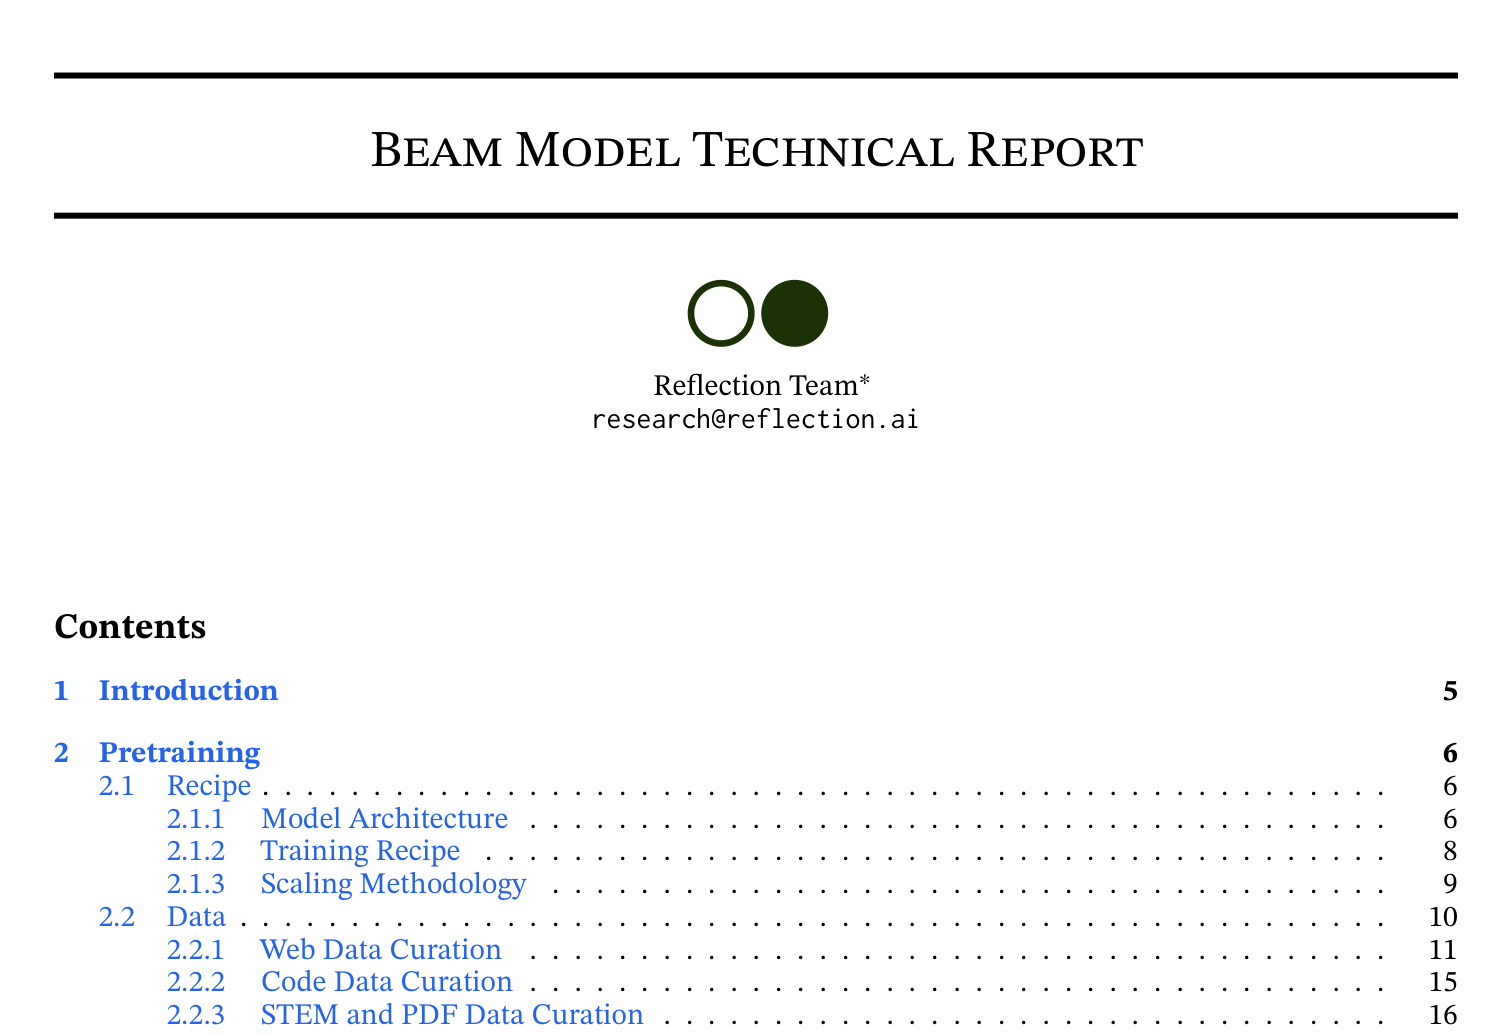
\includegraphics[width=9.8cm]{figures/beam-intro-report-opening.png}}};
  \draw[black!20,line width=.5pt] (2.5,-.1) -- (2.5,2.35)
    -- (12.3,2.35) -- (12.3,-.1);
\end{tikzpicture}
\end{center}
\end{minipage}};
\end{scope}
\end{tikzpicture}
